\documentclass{ximera}

%% Where to look for inputs
\makeatletter     %% make "@" a letter-character
\def\input@path{  %% When looking for files,
{./}              %% look first at your level
{./coverArt/}     %% then in this folder,
{./introduction/} %% then in this folder,
}
\makeatother      %% make "@" an other-character

%% Where to find images
\graphicspath{                      %% When looking for images, 
{./}                                %% look first at your level,
{./setup/}                          %% then in this folder,
{./graphicsVideosAndInteractives/}  %% then in this folder,
}



% Custom Commands


%% These may change and should be checked! 
\newcommand{\docURL}{\url{https://github.com/ximeraProject/ximeraFirstSteps/ximeraUserManual}}
\newcommand{\testURL}{\url{https://github.com/ximeraProject/tests}}
\newcommand{\experimentalURL}{\url{https://github.com/ximeraProject/experimental}}
\newcommand{\xfsURL}{https://go.osu.edu/xfs}
\newcommand{\xfgURL}{https://go.osu.edu/ximera-flash-grant}

\newcommand{\event}[1]{\def\theevent{#1}}
\newcommand{\theevent}{}


\newif\ifcolor %% for color cover
\colorfalse
\colorlet{bkgndcr}{white}
\colorlet{txtcr}{black}
\colorlet{otherbkgndcr}{white}
\colorlet{othertxtcr}{black}


\usepackage{qrcode} %% For QR Codes
\usepackage[normalem]{ulem} % for strikeout
\usepackage{multicol} % multicols -- PDF only

\makeatletter
%% Make Front style
\newcommand\frontstyle{%
  \def\activitystyle{activity-chapter}
  \def\maketitle{%
                {\flushleft\small\sffamily\bfseries\@pretitle\par\vspace{-1.5em}}%
                {\flushleft\LARGE\sffamily\bfseries\@title \par }%3
                {\vskip .6em\noindent\textit\theabstract\setcounter{problem}{0}\setcounter{section}{0}}%
                \par\vspace{2em}    
                \phantomsection\addcontentsline{toc}{section}{\textbf{\@title}}%
                \setcounter{titlenumber}{0}
}}

\renewcommand\chapterstyle{%
  \def\activitystyle{activity-chapter}
  \normalsize
  %\onecolumn
  \def\maketitle{%
    \addtocounter{titlenumber}{1}%
                    {\flushleft\small\sffamily\bfseries\@pretitle\par\vspace{-1.5em}}%
                    {\flushleft\LARGE\sffamily\bfseries\thetitlenumber\hspace{1em}\@title \par }%
                    {\vskip .6em\noindent\textit\theabstract\setcounter{problem}{0}\setcounter{section}{0}}%
                    \par\vspace{2em}
                    \phantomsection\addcontentsline{toc}{section}{\textbf{\thetitlenumber\hspace{1em}\@title}}%
}}

%% Redefine section and subsection
\renewcommand\section{\@startsection {section}{1}{\z@}%
                                   {-3.5ex \@plus -1ex \@minus -.2ex}%
                                   {2.3ex \@plus.2ex}%
                                   {\boldmath\normalfont\large\bfseries\sffamily}}
\renewcommand\subsection{\@startsection{subsection}{2}{\z@}%
                                     {-3.25ex \@plus -1ex \@minus -.2ex}%
                                     {1.5ex \@plus .2ex}%
                                     {\boldmath\normalfont\large\bfseries\sffamily}}


\renewcommand\paragraph{\@startsection{paragraph}{4}{\z@}%
                                    {3.25ex \@plus1ex \@minus.2ex}%
                                    {-1em}%
                                    {\boldmath\normalfont\normalsize\bfseries\sffamily}}
\makeatother

\title{Set up a xourse}

\author{Bart Snapp}

\begin{document}
\begin{abstract}
  How to set up a xourse
\end{abstract}
\maketitle

% \section{Setting up a Ximera \texttt{xourse}}

Ximera documents can be \textit{glued} together using the \texttt{xourse}
document
class.
A \verb|xourse| file is basically a list of other \verb|ximera| files and even
other \verb|xourse| files.
The \verb|xourse| file for \textit{A First Step in Ximera} can be found here is
\verb!aFirstStepInXimera.tex!, found in the \verb!ximeraFirstSteps! repository.
The \verb!xourse! documentclass specifies information such as the name of the
document, the names fo the authors, a description of the content, a license and
the names of all Ximera \LaTeX\ files comprising
the whole document.

\begin{warning}
  All document and folder names used for Ximera must be web-safe! This means
  all document and folder names:
  \begin{description}
    \item[Must only use alphanumeric English characters] Meaning: a,b, \dots,
      z, A,B, \dots, Z, 0,1, \dots, 9, and hyphen `-' and underscore `\_'
      though the
      last two are discouraged.
    \item[Cannot use use any other characters, including spaces] This means all
      Ximera documents and folders file names must be a single word.
  \end{description}
  This is not a limitation of Ximera, rather it is a rule that nearly all
  web-accessible documents must follow.
\end{warning}

\section{File structure}

While one can write a Ximera document without the use of folders, this quickly
turns into a mess that is difficult to understand and should only be used for
the most basic Ximera content.
To help others (including your future-self) work with larger projects, you
should have a file structure
that helps developers understand where content is stored. We recommend the
following:
\begin{description}
  \item[Group by concept] by having all documents that are closely related in
    idea
    or scope in the same folder. If someone else wants to use your content,
    this will be a one-stop destination for them.
  \item[Descriptive file names] will help you and others understand the
    structure of your repository. Give you documents descriptive file names like:
    \verb!completeTheSquare.tex! or \verb!derivativeRules.tex! rather than
    generic
    names like: \sout{\texttt{chapter1.tex}}, or
    \sout{\texttt{math872ch2sec3.tex}}. Authors find themselves reordering
    their content and generic names are useless for other users.
\end{description}

For the repository \texttt{ximeraFirstSteps} we have the following structure:
\begin{center}%%DIAGRAM OF FILE STRUCTURE
  \scalebox{.7}{
    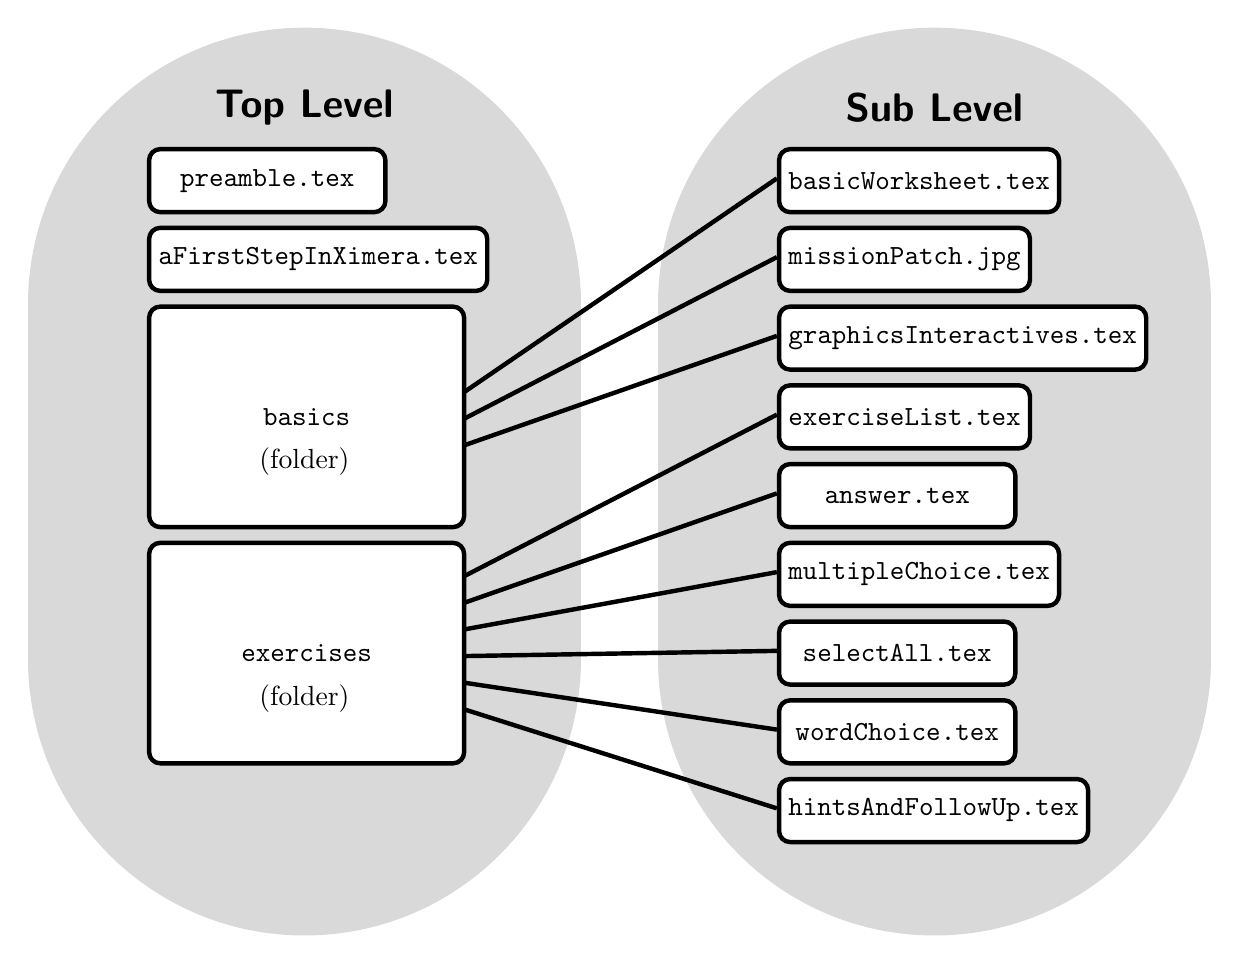
\begin{tikzpicture}
      % Define styles for nodes
      \tikzstyle{document} = [anchor=north west,draw, rounded corners,
      rectangle,
      minimum width=3cm,fill=white, minimum height=.8cm, ultra
      thick,font=\ttfamily]
      \tikzstyle{folder} = [anchor=north west,draw, rectangle, rounded corners,
      minimum width=4cm,fill=white, minimum height=2.8cm, ultra
      thick,font=\ttfamily]

      % Thick grey lines
      \draw[line width=200pt,white!85!black,line cap=round] (2,1) -- (2,-3.5);
      \draw[line width=200pt,white!85!black,line cap=round] (10,1) --(10,-3.5);

      % Connections
      \draw[ultra thick] (2,-1.5) -- (8,2.6);
      \draw[ultra thick] (2,-1.5) -- (8,1.6);
      \draw[ultra thick] (2,-1.5) -- (8,.6);

      \draw[ultra thick] (2,-3.5) -- (8,-.4);
      \draw[ultra thick] (2,-3.5) -- (8,-1.4);
      \draw[ultra thick] (2,-3.5) -- (8,-2.4);
      \draw[ultra thick] (2,-3.5) -- (8,-3.4);
      \draw[ultra thick] (2,-3.5) -- (8,-4.4);
      \draw[ultra thick] (2,-3.5) -- (8,-5.4);

      % Symbols at top
      \node at (2,3.5) {\Large\bf\sffamily  Top Level};
      \node at (10,3.5) {\Large\bf\sffamily Sub Level};

      % Define the folders at top level
      \node[document] at (0,3) {preamble.tex};
      \node[document] at (0,2) {aFirstStepInXimera.tex};
      \node[folder] at (0,1) {basics};
      \node[] at (2,-1) {(folder)};
      \node[folder] at (0,-2) {exercises};
      \node[] at (2,-4) {(folder)};

      % Define the documents in the basics folder
      \node[document] at (8,3) {basicWorksheet.tex};
      \node[document] at (8,2) {missionPatch.jpg};
      \node[document] at (8,1) {graphicsInteractives.tex};

      % Define the documents in the exercises folder
      \node[document] at (8,0) {exerciseList.tex};
      \node[document] at (8,-1) {answer.tex};
      \node[document] at (8,-2) {multipleChoice.tex};
      \node[document] at (8,-3) {selectAll.tex};
      \node[document] at (8,-4) {wordChoice.tex};
      \node[document] at (8,-5) {hintsAndFollowUp.tex};

    \end{tikzpicture}}
\end{center}
We've left some files out of this diagram; regardless, you should be able to
goto
\begin{center}
  \url{https://github.com/ximeraProject/ximeraFirstSteps}
\end{center}
and witness this file structure. At the top level of the repository, we have
the documents \verb!preamble.tex! and \verb!aFirstStepInXimera.tex! along with
the folders \verb!basics! and \verb!exercises!. Inside \verb!basics!, we have
two activities and a JPG that is required by one of them. Inside
\verb!exercises!
we have all the practice exercises.
Ideally a document's parent folder would contain everything that document needs
to compile, except for perhaps the preamble, and we address this below.

A consistent and well thought out set up will allow you and others to easily
understand and modify your
content for years to come.

\begin{warning}
  Every \verb!*.tex! file in the repository with a \verb!\documentclass!
  \textbf{must} compile for online deployment.
\end{warning}

\section{Including with \texttt{\textbackslash activity} and
  \texttt{\textbackslash practice}}

Once you have some files and a basic directory structure, you can add them to
the \verb!xourse! document.

\begin{warning}
  The \verb!xourse! document will only be easily accessible online if it
  contains a title,
  abstract, and {\tt\textbackslash maketitle} command.

  If a \verb!xourse! does not contain a title, abstract, and {\tt\textbackslash
      maketitle} it will still be deployed but you will need to know the path
  to the
  file. It will be something like:
  \begin{center}
    \tt https://ximera.osu.edu/YOUR-COURSE-NAME/PATH-TO-YOUR-FILE
  \end{center}
  It is important that there is no trailing `/' as
  \begin{itemize}
    \item \url{https://ximera.osu.edu/moooculus} is correct but
    \item \sout{\url{https://ximera.osu.edu/moooculus/}} is not.
  \end{itemize}
\end{warning}

There are two different commands we use to add
\verb!ximera! documents to a \verb!xourse! file:
\begin{description}
  \item[\tt\bfseries\textbackslash activity] is for including Ximera documents
    that
    \textbf{include a title,
      abstract, and \tt\bfseries\textbackslash maketitle}. They will be
    represented by
    their title
    online. This command is typically used for worksheets and sections of
    textbooks.
  \item[\tt\bfseries\textbackslash practice] is for including Ximera documents
    that \textbf{do
      not include} a title, abstract, and \verb!\maketitle!. They will be
    represented by a number  based on their
    order in \verb!xourse! file. This command is used for lists of exercises
    and problem
    banks.
\end{description}

In \verb!aFirstStepInXimera.tex! we write

\begin{verbatim}
\documentclass{xourse} 
%% Where to look for inputs
\makeatletter     %% make "@" a letter-character
\def\input@path{  %% When looking for files,
{./}              %% look first at your level
{./coverArt/}     %% then in this folder,
{./introduction/} %% then in this folder,
}
\makeatother      %% make "@" an other-character

%% Where to find images
\graphicspath{                      %% When looking for images, 
{./}                                %% look first at your level,
{./setup/}                          %% then in this folder,
{./graphicsVideosAndInteractives/}  %% then in this folder,
}



% Custom Commands


%% These may change and should be checked! 
\newcommand{\docURL}{\url{https://github.com/ximeraProject/ximeraFirstSteps/ximeraUserManual}}
\newcommand{\testURL}{\url{https://github.com/ximeraProject/tests}}
\newcommand{\experimentalURL}{\url{https://github.com/ximeraProject/experimental}}
\newcommand{\xfsURL}{https://go.osu.edu/xfs}
\newcommand{\xfgURL}{https://go.osu.edu/ximera-flash-grant}

\newcommand{\event}[1]{\def\theevent{#1}}
\newcommand{\theevent}{}


\newif\ifcolor %% for color cover
\colorfalse
\colorlet{bkgndcr}{white}
\colorlet{txtcr}{black}
\colorlet{otherbkgndcr}{white}
\colorlet{othertxtcr}{black}


\usepackage{qrcode} %% For QR Codes
\usepackage[normalem]{ulem} % for strikeout
\usepackage{multicol} % multicols -- PDF only

\makeatletter
%% Make Front style
\newcommand\frontstyle{%
  \def\activitystyle{activity-chapter}
  \def\maketitle{%
                {\flushleft\small\sffamily\bfseries\@pretitle\par\vspace{-1.5em}}%
                {\flushleft\LARGE\sffamily\bfseries\@title \par }%3
                {\vskip .6em\noindent\textit\theabstract\setcounter{problem}{0}\setcounter{section}{0}}%
                \par\vspace{2em}    
                \phantomsection\addcontentsline{toc}{section}{\textbf{\@title}}%
                \setcounter{titlenumber}{0}
}}

\renewcommand\chapterstyle{%
  \def\activitystyle{activity-chapter}
  \normalsize
  %\onecolumn
  \def\maketitle{%
    \addtocounter{titlenumber}{1}%
                    {\flushleft\small\sffamily\bfseries\@pretitle\par\vspace{-1.5em}}%
                    {\flushleft\LARGE\sffamily\bfseries\thetitlenumber\hspace{1em}\@title \par }%
                    {\vskip .6em\noindent\textit\theabstract\setcounter{problem}{0}\setcounter{section}{0}}%
                    \par\vspace{2em}
                    \phantomsection\addcontentsline{toc}{section}{\textbf{\thetitlenumber\hspace{1em}\@title}}%
}}

%% Redefine section and subsection
\renewcommand\section{\@startsection {section}{1}{\z@}%
                                   {-3.5ex \@plus -1ex \@minus -.2ex}%
                                   {2.3ex \@plus.2ex}%
                                   {\boldmath\normalfont\large\bfseries\sffamily}}
\renewcommand\subsection{\@startsection{subsection}{2}{\z@}%
                                     {-3.25ex \@plus -1ex \@minus -.2ex}%
                                     {1.5ex \@plus .2ex}%
                                     {\boldmath\normalfont\large\bfseries\sffamily}}


\renewcommand\paragraph{\@startsection{paragraph}{4}{\z@}%
                                    {3.25ex \@plus1ex \@minus.2ex}%
                                    {-1em}%
                                    {\boldmath\normalfont\normalsize\bfseries\sffamily}}
\makeatother %% Loads the graphics path
\author{Wim Obbels \and Bart Snapp}
\title{A First Step in Ximera}
\begin{document}
\begin{abstract}
    A simple collection of Ximera activities, 
    to be deployed online.
\end{abstract}
\maketitle
\activity{basics/basicWorksheet}
\activity{basics/graphicsInteractives}
\practice{exercises/answer}
\practice{exercises/multipleChoice}
\practice{exercises/selectAll}
\practice{exercises/wordChoice}
\practice{exercises/hintsAndFollowUp}
\end{document}
\end{verbatim}
Note how we give the paths to the exercises.

\end{document}
